\section{Ensemble Learning}

\subsection{Bias and Variance}

\begin{center}
    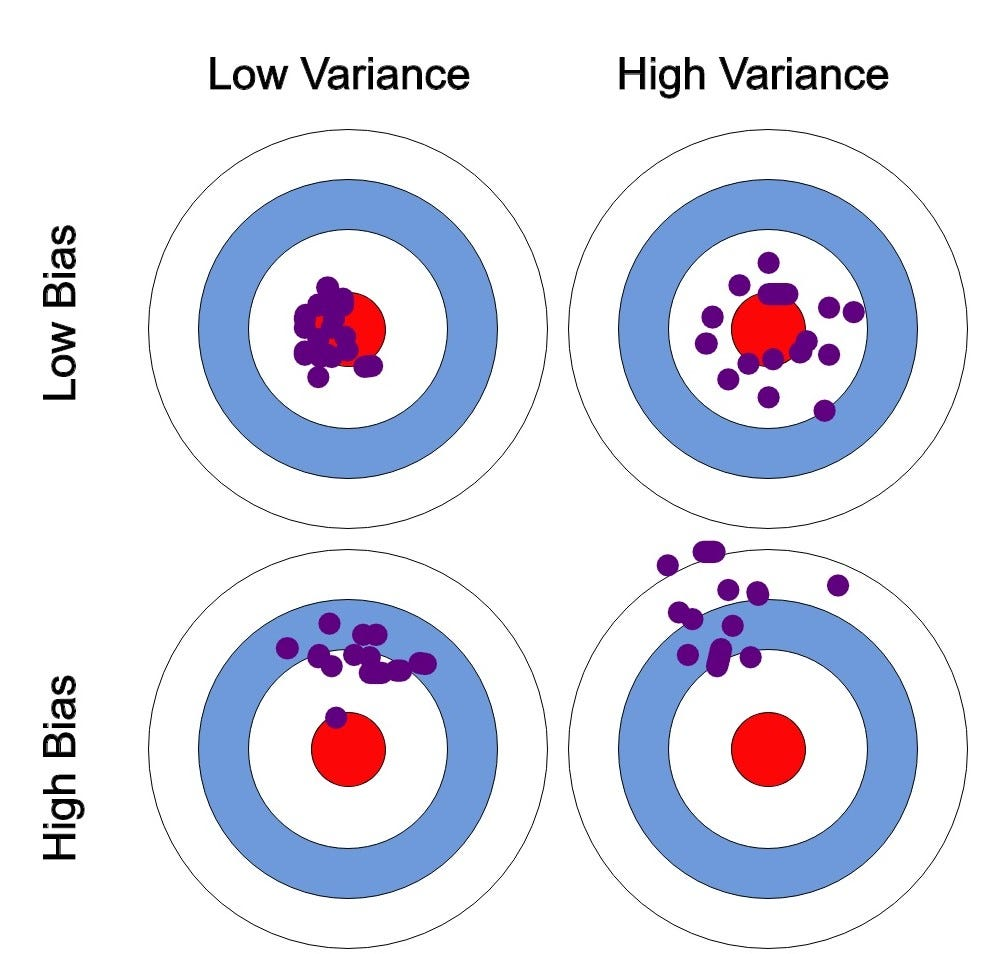
\includegraphics[scale=0.3]{assets/bias_variance.png}
\end{center}

Bias-variance components of error typically show a trade-off. With increasing bias you get decreasing variance and vice versa.

\subsection{Stability}

\begin{itemize}
    \item for a given data distribution \(\mathcal{D}\)
    \item train algorithm \(L\) on the training sets \(S_1, S_2\) sampled from \(\mathcal{D}\)
    \item expect that the model from \(L\) should be the same (or every similar) on both \(S_1\) and \(S_2\)
    \item if so, we say that \(L\) is a stable learning algorithm
    \item otherwise it is unstable
    \item typical stable algorithm: \(k\)NN (for some \(k\))
    \item typical unstable algorithm: decision-tree learning
\end{itemize}

Stable algorithms typically have high bias. Unstable algorithms typically have high variance. But take care to consider effect of parameters. 

\subsection{Ensemble Methods}

In essence, ensemble methods in machine learning have the follow two things in common
\begin{itemize}
    \item they construct multiple, diverse predictive models from adapted versions of the training data (most often reweighted or resampled);
    \item they combine the predictions of these models in some way, often by simple average or voting (possible weighted).
\end{itemize}

Basic idea of ensembles learning schemes: build different ``experts'' and combine their output predictions. Often improved predictive performance but produces output that is very hard to interpret.

\subsubsection{Bagging}

\begin{enumerate}
    \item Sample several training sets of size \(n\) (instead of just having one training set of size \(n\)).
    \item Build a classifier for each training set.
    \item Combine the classifiers' predictions.
\end{enumerate}

Reduces variance by voting/averaging, thus reducing the overall expected error.

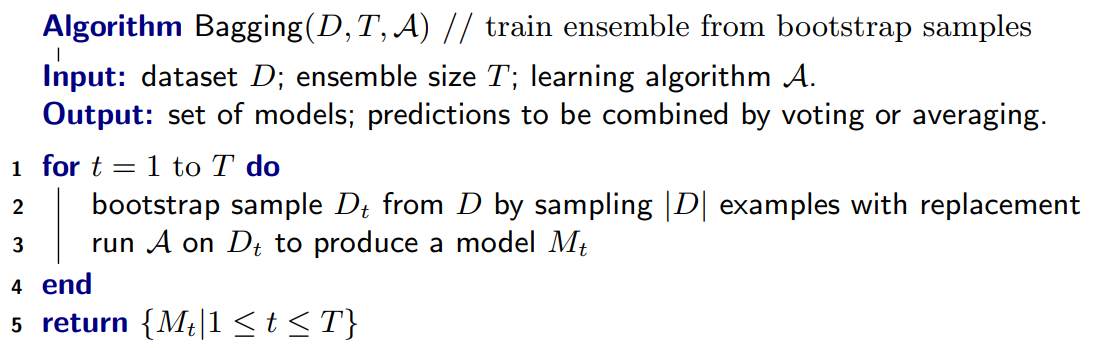
\includegraphics[scale=0.6]{assets/bagging.png}

\subsubsection{Random Forest}

Like bagging for trees, except that the ensemble of tree models is trained from bootstrap samples and random subspaces.

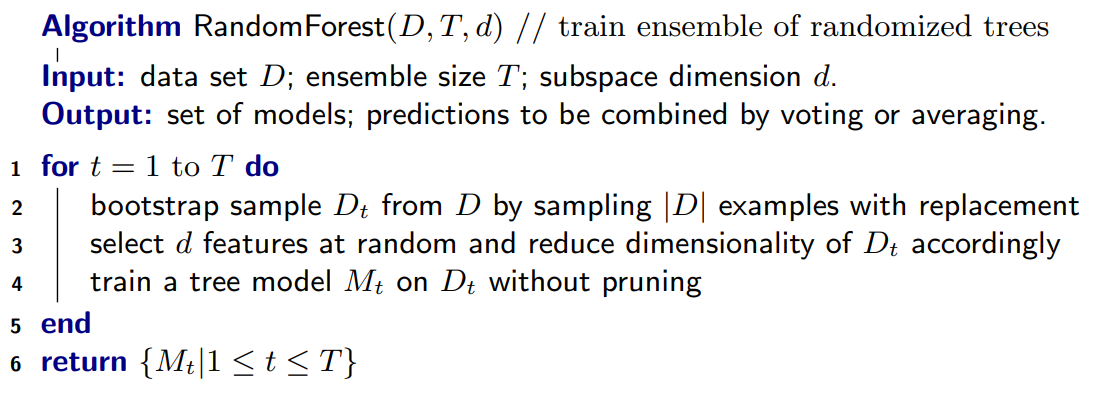
\includegraphics[scale=0.6]{assets/random_forest.png}

\subsubsection{Boosting}

Boosting also uses voting/averaging of an ensemble but each model is weighted according to their performance. An iterative learning procedure, new models are influences by performance of previously built ones.

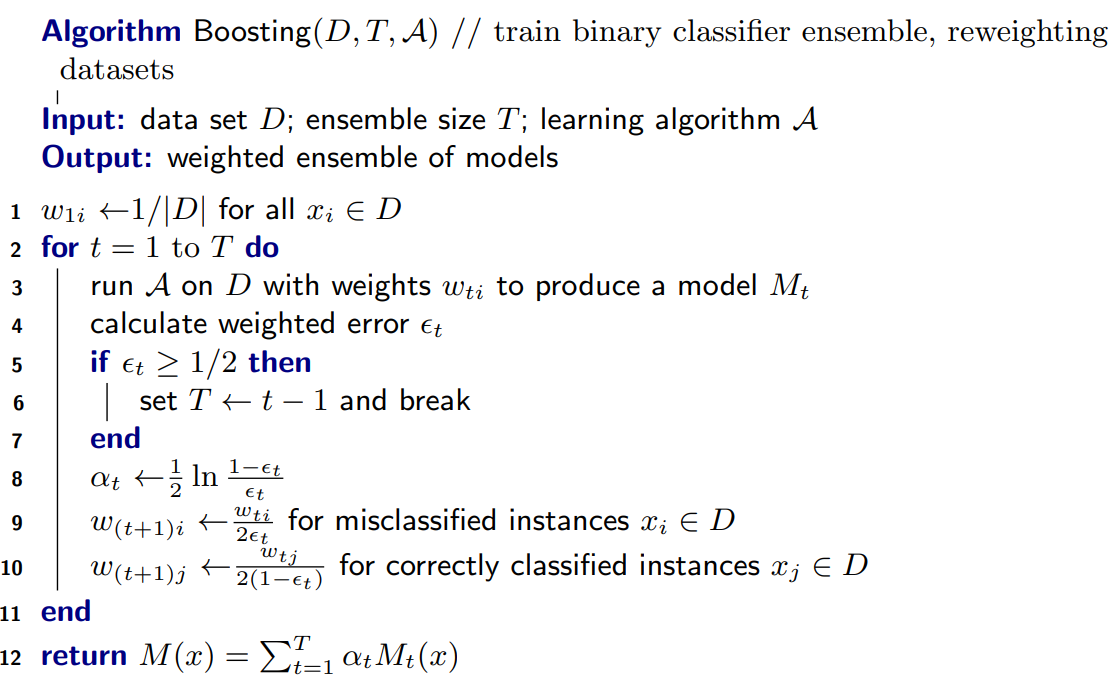
\includegraphics[scale=0.6]{assets/boosting.png}

\subsubsection{Other Ensemble Learning}

Boosting has a more theoretically justified bias and often works better in practice to reduce error, but can be susceptible to very noise data. \\

Many other variants of ensemble learning exists. Gradient Boosting (XGBoost, LightGBM, CatBoost) often the ``off-the-shelf'' method of choice.